\documentclass[10pt]{beamer} % die 10pt sollten festgelegt bleiben, da dies die Groesse der Mathematikschrift etc. beeinflusst
\usepackage[ngerman]{babel}  % deutsche Bezeichnungen und Trennung etc
\usepackage{hyperref}        % interne Hyperlinks
\usepackage[mnf,footuni, headframelogo]{./unirostock/beamerthemeRostock}
\usepackage[utf8]{inputenc}
\usepackage{amsmath}
\usepackage{amssymb}
\usepackage{mathtools}

%cmd
\newcommand{\ol}{\overline} %Kurzform für \overline definiert 
\newcommand{\olsi}[1]{\,\overline{\!{#1}}} % overline short italic
\newcommand{\ols}[1]{\mskip.5\thinmuskip\overline{\mskip-.5\thinmuskip {#1} \mskip-.5\thinmuskip}\mskip.5\thinmuskip} % overline short

%\hyphenation{Online-Back-pro-pa-ga-tions-algo-rithmus Online-Backpropagationsalgorithmus}



%\newcommand{\RR}{\mathbb{R}}
%newcommand{\RRn}{\mathbb{R}^n}

\newcommand{\RR}{\ensuremath{\mathbb{R}}}
\newcommand{\Rnv}{\ensuremath{\mathbb{R}^{n}}}
\newcommand{\Rnn}{\ensuremath{\mathbb{R}^{n\times n}}}

\newcommand{\NN}{\ensuremath{\mathbb{N}}}

\newcommand{\mK}{\ensuremath{\mathcal{K}}}
\newcommand{\mKp}{\ensuremath{\mathcal{K}}^+}
\newcommand{\Code}{\ensuremath{C^{\textnormal{dgl}}}}


%%%%


%%%%%%%%%%%% Festlegung der Titelseite %%%%%%%%%%%%%%%%%%%%%%%%%%%%%%%%%
\title[Datenbankgestützte Erkennung von Mustern in trainierten gefalteten neuronalen Netzen]{Datenbankgestützte Erkennung von Mustern in trainierten gefalteten neuronalen Netzen}

\subtitle{Verteidigung, 14. September 2022}

\author{\textsc{Florian Baldauf}}

\date{14. September 2022}

\institute{Universität Rostock, Institut für Mathematik}

\footinstitute{Mathematisch Naturwissenschaftliche Fakultät, Institut für Mathematik}

\renewcommand{\mylogo}{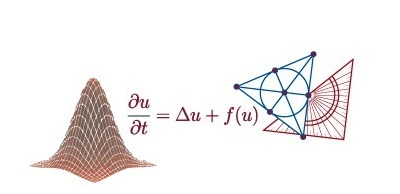
\includegraphics[height=15mm]{institut}}


%%%%%%%%%%%%%%%%%% Los geht's %%%%%%%%%%%%%%%%%%%%%%%%%%%%%%%%%%%%%%%%%
%%%%%%%%%%%%%%%%%%%%%%%%%%%%%%%%%%%%%%%%%%%%%%%%%%%%%%%%%%%%%%%%%%%%%%%
\begin{document}


%%%%%%%%%%%%%%%%%%%%%%%%%%%%%%%%%%%%%%%%%%%%%%%%%%%%%%%%%%%%%%%%%%%%%%%
%%%%%%%%%%%%%%%%%%%%%%%%%%%%%%%%%%%%%%%%%%%%%%%%%%%%%%%%%%%%%%%%%%%%%%%
\begin{frame}% Titelseite
  \titlepage
\end{frame}


%%%%%%%%%%%%%%%%%%%%%%%%%%%%%%%%%%%%%%%%%%%%%%%%%%%%%%%%%%%%%%%%%%%%%%%
%%%%%%%%%%%%%%%%%%%%%%%%%%%%%%%%%%%%%%%%%%%%%%%%%%%%%%%%%%%%%%%%%%%%%%%
\begin{frame}{Ablauf}%{Damit der Hörer auch ein wenig durchsieht}
  \tableofcontents[pausesections]
\end{frame}


%%%%%%%%%%%%%%%%%%%%%%%%%%%%%%%%%%%%%%%%%%%%%%%%%%%%%%%%%%%%%%%%%%%%%%%
%%%%%%%%%%%%%%%%%%%%%%%%%%%%%%%%%%%%%%%%%%%%%%%%%%%%%%%%%%%%%%%%%%%%%%%
\section{Einführung Mathematik und Künstlichen Intelligenz}


\begin{frame}
   \frametitle[]{KI: Erfolg in vielen Disziplinen}
\end{frame}

\begin{frame}
   \frametitle[]{Meine Problemstellungen}
   TODO
\end{frame}
%%%%%%%%%%%% Beispielfolie aus dem BeamerUsersguide %%%%%%%%%%%%%%%%%%%
%%%%%%%%%%%%%%%%%%%%%%%%%%%%%%%%%%%%%%%%%%%%%%%%%%%%%%%%%%%%%%%%%%%%%%%
\subsection{Neuronale Netze}

\begin{frame}
  \frametitle{Erste Ansätze}
Ideen von McCulloch und Pitts (1943):
\begin{itemize}
   \item Entwicklung einer algorithmischen Beschreibung des Lernens
   \item menschliche Gehirn als Vorbild $\rightarrow$ das abstrakte Neuron
\end{itemize}
\end{frame}

\begin{frame}
   \frametitle[]{Das Neuron}
   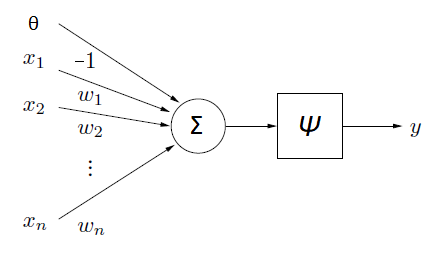
\includegraphics[width=0.9\textwidth]{pics/perzeptron.png}
\end{frame}

\begin{frame}
   \begin{block}{Definition (Neuron)}
      \label{def_neuron}
      Für eine gegebene Funktion $\phi: \RR \rightarrow \RR$, einen Vektor $w \in \Rnv$ und ein Skalar $b \in \RR$ wird die Funktion 
      \[ \
      \Phi: \RR^n \rightarrow \RR, \; \; \; x \mapsto \phi(w^T x -b)=:y,
      \]
      \textit{Neuron} genannt.
   \end{block}
   \pause
   Mögliche Aktivierungsfunktionen sind:
   \begin{align*}
      \text{Identität}: \; \;\phi(x)&=x, \\
      \text{Logistische Funktion}: \; \;\phi(x)&=\frac{1}{1+\mathrm{e}^{-x}}, \\
      \text{ReLU (rectified linear unit)}: \; \;\phi(x)&=\max\{0,x\}.
  \end{align*}
\end{frame}

\begin{frame}
   Die Verknüpfung von Neuronen zu Netzen führt zur Komposition von affin linearen Abbildungen und Aktivierungsfunktionen.
   \pause

   Ein Beispiel(Quelle Gitta Kutyniok \cite{})
   \begin{equation*}
      \Phi: \RR^3 \rightarrow \RR^2, \; \; \Phi(x)=W^{(2)}\phi(W^{(1)}x-b^{(1)})-b^{(2)}
   \end{equation*}
   
   \begin{minipage}[c]{0.35\textwidth}
      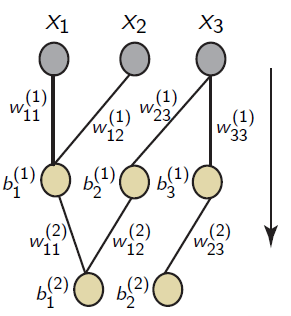
\includegraphics[width=\textwidth]{pics/FF_sparse.png}
      \end{minipage}
      \begin{minipage}[c]{0.3\textwidth}
         \begin{align*}
            W^{(1)} &= \begin{pmatrix}
               w_{11}^{(1)} & w_{12}^{(1)} &0 \\
               0 &0 &w_{23}^{(1)} \\
               0 &0 &w_{33}^{(1)} \\
            \end{pmatrix} \\
            W^{(2)} &= \begin{pmatrix}
               w_{11}^{(2)} & w_{12}^{(1)} &0 \\
               0 &0 &w_{23}^{(2)}
            \end{pmatrix}
         \end{align*}  
      \end{minipage}
\end{frame}

\begin{frame}
   \frametitle[]{Neuronale Netze}
   \begin{block}{Definition (Vorwärtsgerichtetes neuronales Netz(FNN))}
      Seien 
      \begin{itemize}
         \item $s_0 \in \mathbb{N}$: Dimension der Eingabeschicht,
         \item $L$: Anzahl der Schichten, 
         \item $\phi$: eine (nichtlineare) Aktivierungsfunktion,
         \item Neuronen: $T_{\ell}: \RR^{s_{\ell-1}} \rightarrow \RR^{s_\ell}, \; \ell=1, \ldots L, \; \text{mit} T_{\ell}(x)=W^{(\ell)}x+b^{(\ell)}$
      \end{itemize}
      \pause
      Dann ist $\Phi: \RR^{s_0} \rightarrow \RR^{s_L}$ durch die Komposition 
      \begin{equation*}
         \Phi(x)=T_{L} \circ \phi \circ T_{L-1} \circ \phi \circ \ldots \circ \phi \circ T_1(x), \; x \in \RR^{s_0}
      \end{equation*}
      erklärt. Der Vektor $y:=\Phi(x)$ wird Ausgabe des (tiefen) FNN genannt.
   \end{block}
\end{frame}

\begin{frame}
   \frametitle[]{Veranschaulichung}
   \begin{figure}
      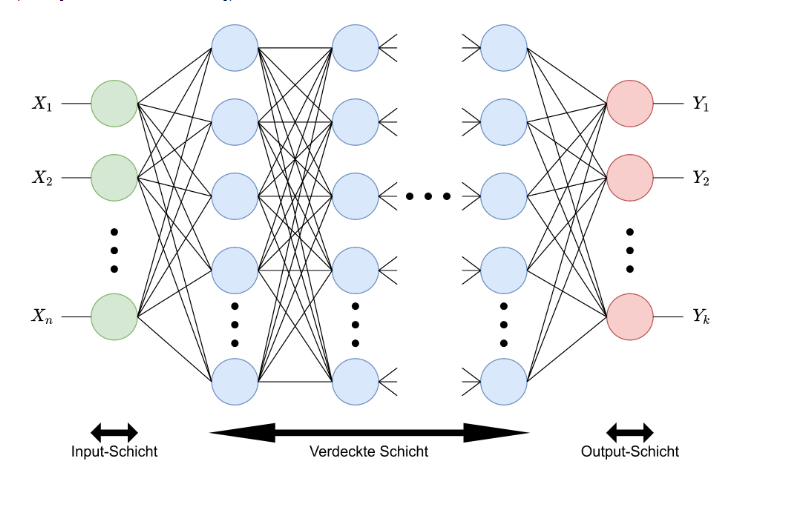
\includegraphics[width=0.8\textwidth]{pics/full_FFN.png}
      \caption[]{Die Abbildung ist aus Fenske\cite[]{fenske} entnommen.}
   \end{figure}
\end{frame}

%%%%%%%%%%%% Beispielfolie zum Mathemodus %%%%%%%%%%%%%%%%%%%%%%%%%%%%%
%%%%%%%%%%%%%%%%%%%%%%%%%%%%%%%%%%%%%%%%%%%%%%%%%%%%%%%%%%%%%%%%%%%%%%%
\subsection{Erkennung von Mustern}
\begin{frame}{Überwachtes Lernen}{Klassifikation von Objekten mithilfe vonFFN}
Gegeben: 
\begin{itemize}
   \item Menge $\mathcal{M}=\{x_i \in \RR^n \, : \, 1 \leq i \leq m\}$,
   \item Funktion $f: \mathcal{M} \rightarrow \{1, \ldots k\}$,
   \item also eine endliche Menge von Tupeln der Form $(x_i, f(x_i))_{i=1}^m$, auch Trainingsmenge $\mathcal{T}$ genannt.
\end{itemize} 
\pause
Gesucht: affin lineare Funktionen $(T_{\ell})_{\ell=1}^L=(W^{(\ell)} \cdot + b^{(\ell)})_{\ell=1}^L$ (oft Netzeingabe, Input des Neurons) sodass das Problem

\begin{equation*}
   \underset{(W^{(\ell)}, b^{(\ell)})_\ell}{\min} \sum_{i=1}^m \mathcal{E}(\Phi(x_i),f(x_i)) +\lambda \mathcal{R}((W^{(\ell)}, b^{(\ell)})_l)
\end{equation*}
gelöst wird. Hier ist $\mathcal{E}(\mathcal{T},\mathcal{W})$ eine wählbare Zielfunktion.
\end{frame}

\begin{frame}
   \frametitle{Training von FFN}
   Training mithilfe des Gradientenverfahren als iteratives Verfahren mit dem langfristigen Ziel $\Phi(x_i) \approx f(x_i)$ für die Testdaten 
   
   $\rightarrow$ Backpropagation mit mehrdimensionaler Kettenregel
   
   Sei $\mathcal{W}=\{(W^{(\ell)},b^{(\ell)}) \, : \, 1 \leq \ell \leq L\}$ die Menge der Modellparameter.

   Idee: 
   \begin{itemize}
      \pause
      \item Bestimme Gradient $\Delta_n=\nabla_{\mathcal{W}} \mathcal{E}(\mathcal{T},\mathcal{W})$,
      \pause
      \item Aktualisiere Parameter $\mathcal{W}_{n+1}= \mathcal{W}_n+ \lambda \Delta_n$,
      \pause
      \item solange ein Abbruchkriterium nicht erfüllt ist.
   \end{itemize} 

\end{frame}

\begin{frame}
   Wähle Zielfunktion $\mathcal{E}(x,\mathcal{W})= \frac{1}{2} \sum_{(x,c) \in \mathcal{T}} ||y-t||_2^2$ mit dem Zielvektor $t=t(x,c)$. Online-Backpropagation $\rightarrow E_x=\frac{1}{2} \sum_{k=1}^{s_L} (y_k-t_k)^2.$
   \pause
   \begin{block}{Satz (Online-Backpropagation)}
   Seien mit $w_{j,i}^{(\ell)}$ und $b_j^{(\ell)}$ lernbare Parameter der Schicht $\ell$ bezeichnet.

   Dann gilt 
   \begin{equation*}
       \Delta w^{(\ell)}_{j,i}= \frac{\partial E_x}{\partial w^{(\ell)}_{j,i}}= \delta^{(\ell)}_j z^{(\ell-1)}_i, \; \;
       \Delta b^{(\ell)}_{j}= \frac{\partial E_x}{\partial b^{(\ell)}_{j}}= \delta^{(\ell)}_j
   \end{equation*}
   mit 
   \begin{equation*}
       \delta^{(\ell)}_j=
       \begin{cases}
           (y_j-t_j) \phi'(T^{(L)}_j), &\text{wenn $j$ ein Ausgabeneuron ist}, \\
           \left(\sum_{k} \delta^{(\ell+1)}_k w^{(\ell+1)}_{k,j}\right) \phi'(T_j^{(\ell)}), &\text{sonst}.
       \end{cases}
   \end{equation*}
\end{block} 
\end{frame}

\begin{frame}
   \frametitle[]{Lineare Algebra}
   Kompakte Darstellung: 

   \begin{equation*}
      \Delta W^{(\ell)}= \delta^{(\ell)} \cdot z^{{(\ell-1)}^T}, \; \;
      \Delta b^{(\ell)}= \delta^{(\ell)}  
   \end{equation*}
  mit 
  \begin{equation*}
      \delta^{(\ell)}=
      \begin{cases}
          (y-t) \odot \phi'(T^{(L)}), &\text{wenn $\ell=L$}, \\
          \left(W^{{(\ell+1)}^T} \delta^{(\ell+1)}\right) \odot \phi'(T^{(\ell)}), &\text{wenn $\ell \in \{1, \ldots L-1\}$},
      \end{cases}
  \end{equation*}
  und dem dyadischen Produkt, Matrixvektorprodukt sowie die elementweise Multiplikation.
\end{frame}

\begin{frame}{Klassifikation von Grauwertbildern}{Ein paar Probleme}

   Beispiel: Bild ($1000 \times 1000$) und jedes Pixel als Merkmal

   FFN mit 10 Ausgabeneuronen $\rightarrow$ $10^7+10$ freie Parameter

   $\rightarrow$ Reduzierung durch Parameter Sharing, sparse connectivity

   Korrelationen zwischen benachbarten Neuronen?
   
   $\rightarrow$ Filter, zum Beispiel zur Kantendetektierung
\end{frame}

\section{Gefaltete neuronale Netze (CNN)}
\subsection{Funktionsweise}
\begin{frame}{Convolutional Neural Networks (CNN)}
Unterschiede zu klassischen FFN:
\pause
\begin{itemize}
   \item Berechnung der Netzeingabe.
   \pause 
   \item Mehrere Neuronen teilen sich Gewichte.
   \pause
   \item Es liegt kein vollständiger Graph vor.
\end{itemize}
\pause
$\rightarrow$ Reduzierung der Parameteranzahl

$\rightarrow$ Anpassung der Vorwärts- und Rückwärtsrechnung. 

\end{frame}

\begin{frame}{Convolutional Neural Networks (CNN)}{vs. FFN}
   \begin{figure}
      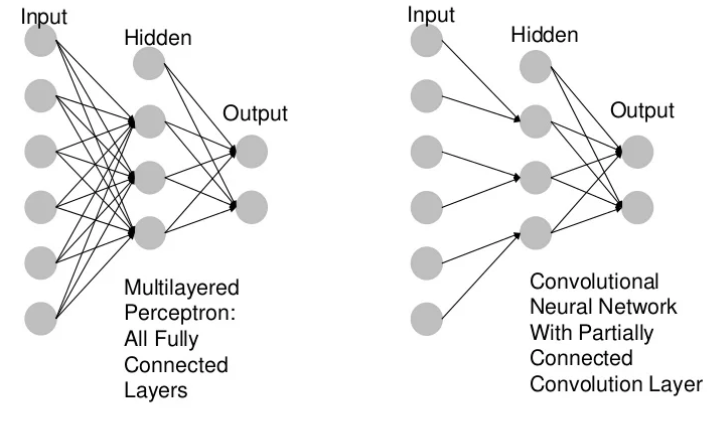
\includegraphics[width=0.75\textwidth]{pics/FFN_vs_CNN.png}
      \caption[]{Architektur von FFN(links) und CNN(rechts). Die Abbildung wurde aus Bhandare\cite{bhandare} entnommen.}
   \end{figure}
\end{frame}

\begin{frame}{Convolutional Neural Networks (CNN)}{Arbeitsweise}
   \begin{figure}
      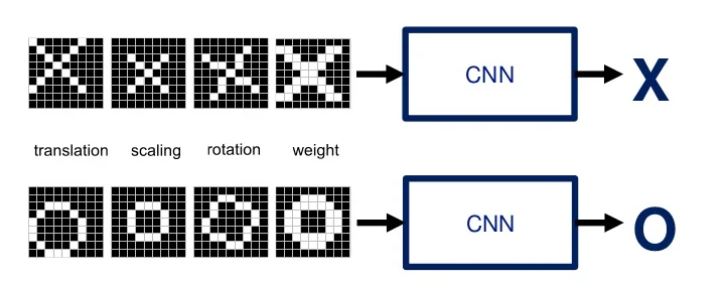
\includegraphics[width=1\textwidth]{pics/arbeitsweise.png}
      \caption{Klassifikation von Grauwertbildern durch CNN. Die Abbildung wurde aus Bhandare\cite{bhandare} entnommen.}
   \end{figure}
\end{frame}

\begin{frame}{Convolutional Neural Networks (CNN)}{Aufbau}
   \begin{itemize}
      \pause
      \item Faltungsschicht: Für Neuronen, welche sich lokal in kleinen Regionen befinden, werden Skalarprodukte mit lernbaren Gewichten (Kernen) berechnet $\rightarrow$ Merkmalskarten.
      \pause
      \item Aktivierungsschicht: Eine Aktivierungsfunktion, z.B. ReLU, wird elementweise auf die Neuronenaktivierungen der Karten angewendet.
      \pause
      \item Pooling-Schicht: Durch sogenanntes downsampling wird die räumliche Dimensionen der Merkmalskarten verringert.
      \pause
      \item FFN: Ein Vorwärtsgerichtetes Netz wird benutzt, um die Klassifikation zu berechnen.
   \end{itemize}
\end{frame}

\begin{frame}{Convolutional Neural Networks (CNN)}{Faltung}
   \begin{block}{Definition (Matrixfaltung)}
      Seien Matrizen $X \in \RR^{h \times b}$ und $K \in \RR^{k \times k}$ gegeben($k$ ungerade). Mit
      \begin{equation*}
          \label{eq:valid_cross}
          Y_{i,j}=\sum_{u=-l}^l \sum_{v=-l}^l X_{i+u,j+v}K_{u,v}
      \end{equation*}
      und $X_{i,j}=0$ für $i \notin [h]$ und $j \notin [b]$ wird die Matrixfaltung $Y= X \ast K \in \RR^{h \times b}$ definiert. Dabei wird $K$ speziell indiziert. Es ist $l=\lfloor k/2 \rfloor$.
   \end{block}
\end{frame}

\begin{frame}{Convolutional Neural Networks (CNN)}{Kerne/Filter}
   Ist beispielsweise $k=3$, so ist $K \in \RR^{3 \times 3}$ durch
    \begin{equation*}
        K=\begin{pmatrix}
            K_{-1,-1} &K_{-1,0} &K_{-1,1} \\
            K_{0,-1} &K_{0,0} &K_{0,1}  \\
            K_{1,-1} &K_{1,0} &K_{1,1} 
        \end{pmatrix}
    \end{equation*} und $K^{rot180}$ durch

    \begin{equation*}
        K^{rot180}=\begin{pmatrix}
            K_{1,1} &K_{1,0} &K_{1,-1} \\
            K_{0,1} &K_{0,0} &K_{0,-1}  \\
            K_{-1,1} &K_{-1,0} &K_{-1,-1} 
        \end{pmatrix}
    \end{equation*}
    gegeben.
\end{frame}

\begin{frame}{Convolutional Neural Networks (CNN)}{Veranschaulichung der Merkmalsextraktion}
   Strides $s_x=s_y=1$, ohne zero padding, $k=3$.
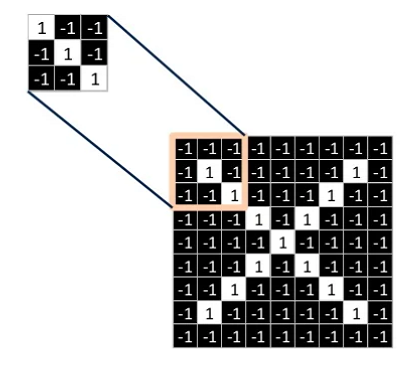
\includegraphics[width=0.55\textwidth]{pics/1window.png}
\end{frame}


\begin{frame}{Convolutional Neural Networks (CNN)}{Veranschaulichung der Merkmalsextraktion}
   Strides $s_x=s_y=1$, ohne zero padding, $k=3$.
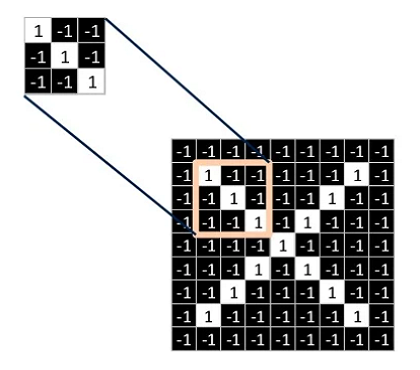
\includegraphics[width=0.55\textwidth]{pics/4window.png}
\end{frame}

\begin{frame}{Convolutional Neural Networks (CNN)}{Ergebnis einer Faltung}
   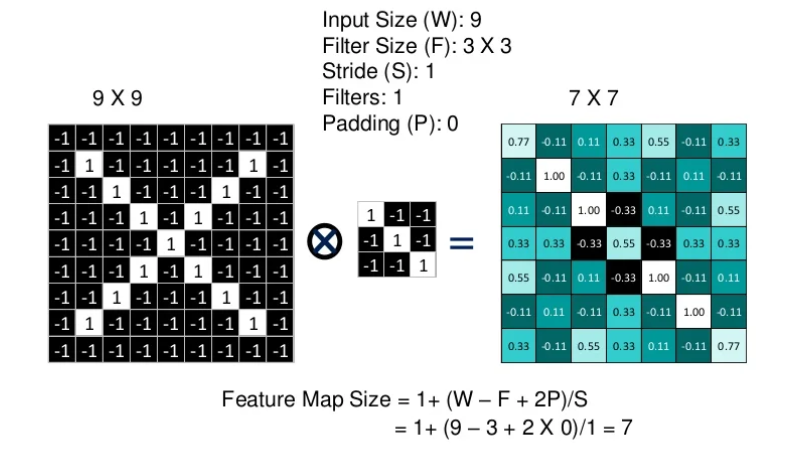
\includegraphics[width=1\textwidth]{pics/sum_cnn.png}
\end{frame}

\begin{frame}{Convolutional Neural Networks (CNN)}{Mehrere Filter}
   \begin{figure}
   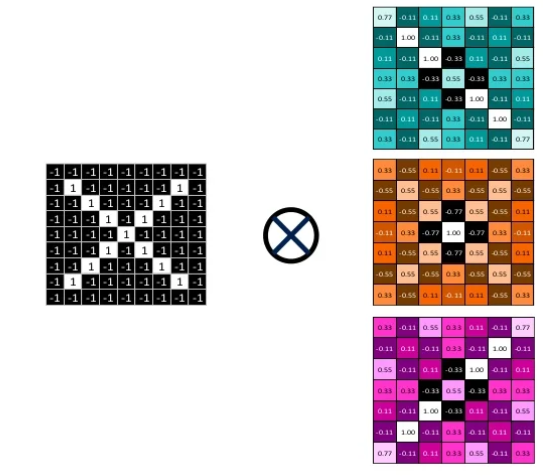
\includegraphics[width=0.65\textwidth]{pics/sum_cnn_multipleK.png}
\end{figure}
\end{frame}

\begin{frame}{Convolutional Neural Networks (CNN)}{Aktivierung}
   \begin{figure}
      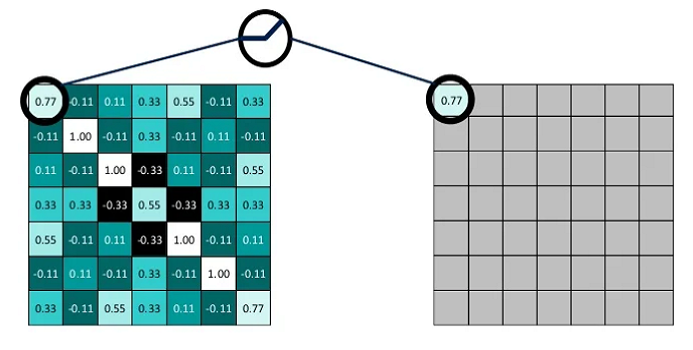
\includegraphics[width=0.95\textwidth]{pics/relu1.png}
   \end{figure}
\end{frame}

\begin{frame}{Convolutional Neural Networks (CNN)}{Aktivierung}
   \begin{figure}
      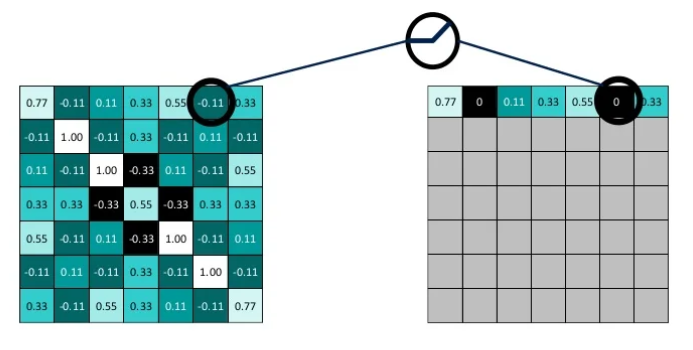
\includegraphics[width=0.95\textwidth]{pics/relu2.png}
   \end{figure}
\end{frame}

\begin{frame}{Convolutional Neural Networks (CNN)}{Pooling}
   Pooling mit Schrittweiten $p_x=p_y=2$, Stride $s_x=s_y=2$ 
   \begin{figure}
      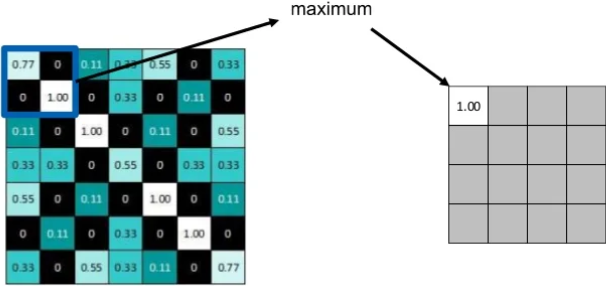
\includegraphics[width=0.85\textwidth]{pics/pool1.png}
   \end{figure}
\end{frame}

\begin{frame}{Convolutional Neural Networks (CNN)}{Pooling}
   Pooling mit Schrittweiten $p_x=p_y=2$, Stride $s_x=s_y=2$ 
   \begin{figure}
      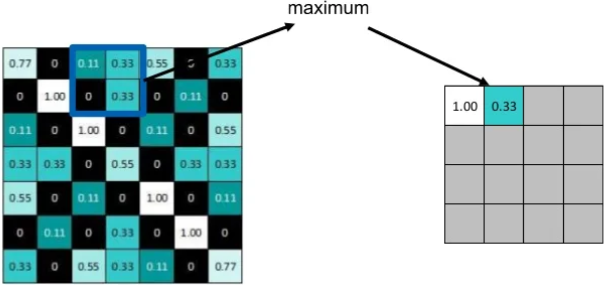
\includegraphics[width=0.85\textwidth]{pics/pool2.png}
   \end{figure}
\end{frame}

\begin{frame}{Convolutional Neural Networks (CNN)}{Pooling}
   Pooling mit Schrittweiten $p_x=p_y=2$, Stride $s_x=s_y=2$ 
   \begin{figure}
      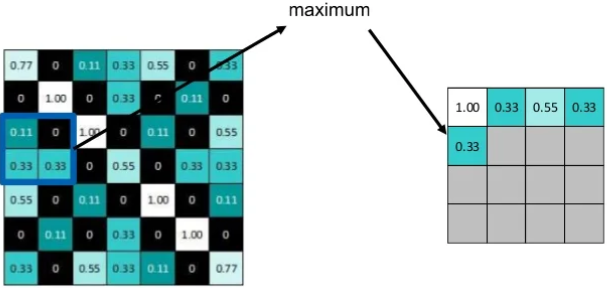
\includegraphics[width=0.85\textwidth]{pics/pool3.png}
   \end{figure}
\end{frame}

\begin{frame}{Convolutional Neural Networks (CNN)}{Kombination von Schichten}
   \begin{figure}
      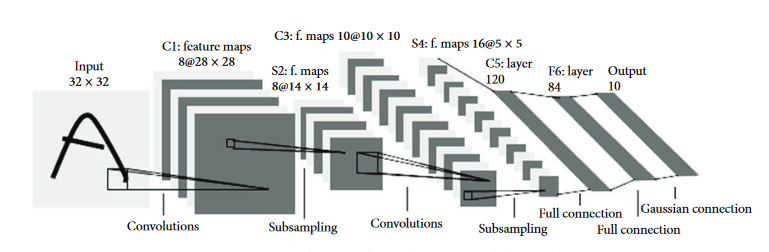
\includegraphics[width=1\textwidth]{pics/lecun5.png}
      \caption{Abgebildet ist die LeNet-5-Architektur\cite{lecun} zur Erkennung von Ziffern aus dem MNIST-Datensatz.} 
   \end{figure}
\end{frame}

\begin{frame}{Convolutional Neural Networks (CNN)}{Mathematische Beschreibung}
Arraydarstellung:  Grauwertbild $X \in \RR^{h \times b \times 1}$,
    Kern $K \in \RR^{z_{out} \times z_{in} \times k \times k}$
\pause
\begin{block}{Definition (Gefaltete Netzeingabe)}
   Die Funktion 
    \begin{equation*}
        \Psi_{conv}^{K,b}: \RR^{\cdot \times \cdot \times z_{in}} \rightarrow \RR^{\cdot \times \cdot\times z_{out}}
    \end{equation*}
    mit
    \begin{equation*}
        \Psi_{conv}^{K,b}(X)_{:,:,q}:= \sum_{p=1}^{z_{in}} \alpha_{qp} \left(K_{q,p,:,:} \ast X_{:,:,p} \right) +b_q, \; \forall q \in [z_{out}]
    \end{equation*}
    wird gefaltete Netzeingabe bezeichnet.
\end{block}
\end{frame}

\begin{frame}{Convolutional Neural Networks (CNN)}{Mathematische Beschreibung}
   \begin{block}{Definition (Faltungsschicht, vgl. Grüning\cite{gruening})}
      Ist $\Psi_{conv}^{K,b}$ eine gefaltete Übertragungsfunktion und $\psi$ eine Aktivierungsfunktion, so wird das Paar $(\Psi_{conv}^{K,b}, \psi)$ als Faltungsschicht $\mathcal{S}_{conv}$ bezeichnet. Für eine sogenannte Eingabekarte $X \in \RR^{\cdot \times \cdot \times z_{in}}$ ist die Ausgabe $Y \in \RR^{\cdot \times \cdot \times z_{out}}$ der Schicht $\mathcal{S}_{conv}$ durch
    \[Y=\psi \circ \Psi_{conv}^{K,b}(X)= \psi\left(\Psi_{conv}^{K,b}(X)\right)
        \] 
        gegeben. Die Matrizen $Y_{:,:,p}$ werden für $1 \leq p \leq z_{out}$ Merkmalskarten genannt. Weiter bezeichne $\Psi_{conv}^{K^{},b^{},\psi_{}}$ die Faltungsschicht $\mathcal{S}_{conv}$ mit $\Psi_{conv}^{K^{},b^{},\psi_{}}(X):= \psi_{} \left(\Psi_{conv}^{K^{},b^{}}(X)\right)$.
   \end{block}
\end{frame}

\begin{frame}{Convolutional Neural Networks (CNN)}{Mathematische Beschreibung}
   Analog werden Pooling-Schichten mit symmetrischen Pooling-Funktionen definiert. Die Kombination mit einem FFN gelingt durch die Flatten-Operation:

   \begin{block}{Definition (Flatten-Schicht)}
      Sei $X \in \RR^{n_1 \times n_2 \times n_3}$. Dann wird die Funktion $T_f:\RR^{n_1 \times n_2 \times n_3} \rightarrow \RR^{n_1 \cdot n_2 \cdot n_3}$ mit 
    \begin{equation*}
        T_f(X)_{(i-1) \cdot (n_2 \cdot n_3)+(j-1) \cdot n_3+k}:= X_{i,j,k}, \; \; \forall i \in [n_1],\; j \in [n_2],\; k \in [n_3]
    \end{equation*}
    Flatten-Funktion genannt. Die mehrdimensionale Eingabe wird also in einen Vektor umgewandelt.
   \end{block}
\end{frame}

\begin{frame}{Convolutional Neural Networks (CNN)}{Kombination von Schichten}
   \begin{figure}
      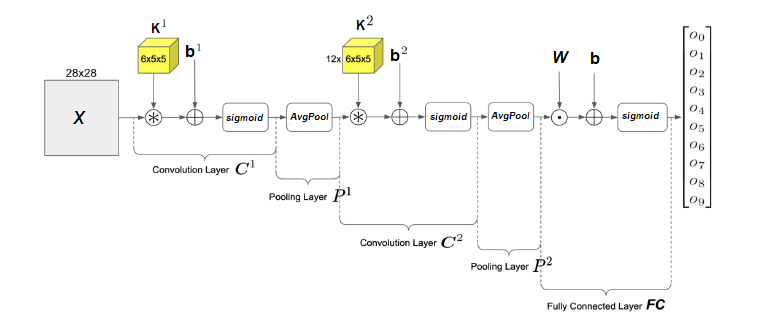
\includegraphics[width=1\textwidth]{pics/modell_arch_anp.png}
      \caption{Zu sehen ist eine CNN-Architektur zur Erkennung von Ziffern.} 
   \end{figure}
\end{frame}
\subsection{Backpropagation}
\begin{frame}{Convolutional Neural Networks (CNN)}{Backpropagation}
 
   Die Aktivierung einer Merkmalskarte $j$ an der Stelle $(x,y)$ lässt sich mit der Matrixfaltung komponentenweise als
   \begin{equation*}
       y_j^{(\ell)}(x,y) =\psi \left(\sum_{i=1}^{z_{in}} \sum_{(u,v) \in F} y_i^{(\ell-1)}(x+u,y+u)\,  w_{j,i}^{(\ell)}(u,v) +b_j^{(\ell)}\right)
   \end{equation*}   
   schreiben, wobei $j \in [z_{out}]$. Beachte $K^{(\ell)}_{j,i,u,v}= w_{j,i}^{(\ell)}(u,v)$, $F=\{(u,v): \; -l \leq u,v \leq l\}$ und $y^{(\ell)} \in \RR^{z_{out} \times \cdot \times \cdot}$.
   \pause

   Vergleich zu FFN:
   \begin{equation*}
      y_j^{(\ell)}(1,1) =\psi \left(\sum_{i=1}^{s_{\ell-1}} y_i^{(\ell-1)}(1,1)\,  w_{j,i}^{(\ell)} +b_j^{(\ell)}\right)
  \end{equation*} 

\end{frame}

\begin{frame}{Convolutional Neural Networks (CNN)}{Backpropagation}
   Der Gradient von $w_{j,i}^{(\ell)}$ ergibt sich als Summe über alle beteiligten Pixel $(x,y)$ der Merkmalskarte $j$, also
\begin{equation*}
    \label{eq:CNN_K_grad}
    \Delta w_{j,i}^{(\ell)}(u,v)= \sum_{(x,y)} \left(\delta_j^{(\ell)}(x,y)  y_i^{(\ell-1)}(x+u,y+v)\right)
\end{equation*} und 
\begin{equation*}
   \Delta b_j^{(\ell)}= \sum_{(x,y)} \delta_j^{(\ell)}(x,y).
\end{equation*}
\end{frame}

\begin{frame}{Convolutional Neural Networks (CNN)}{Veranschaulichung}
   \begin{figure}
   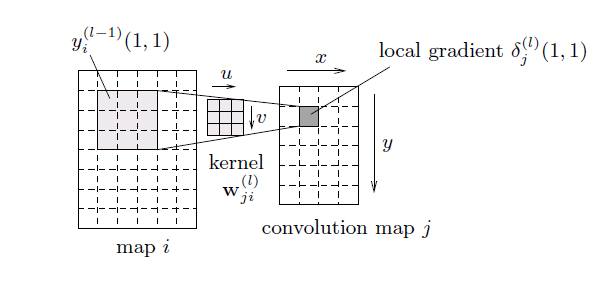
\includegraphics[width=0.95\textwidth]{pics/backprop_dudiss.png}\caption[Rückwärtsrechnung bei CNN]{Es ist die Rückwärtsrechnung bei Faltungsschichten dargestellt. Die Abbildung wurde aus \cite{du_diss} entnommen.}
   \end{figure}
\end{frame}

\begin{frame}{Convolutional Neural Networks (CNN)}{Vergleich Backpropagation}
   CNN:
   \begin{align*}
      \label{eq:CNN_K_grad}
      \Delta w_{j,i}^{(\ell)}(u,v)&= \sum_{(x,y)} \left(\delta_j^{(\ell)}(x,y)  y_i^{(\ell-1)}(x+u,y+v)\right) \\
      \Rightarrow \Delta W_{j,i}&= y_i^{(\ell-1)} \ast \delta_j^{(\ell)}, \; \;
     \Delta b_j^{(\ell)}= \sum_{(x,y)} \delta_j^{(\ell)}(x,y).
  \end{align*}

  \pause
  FFN:
  \begin{align*}
   \Delta w^{(\ell)}_{j,i}&= z^{(\ell-1)}_i \delta^{(\ell)}_j\\
   \Rightarrow \Delta W^{(\ell)}&= \delta^{(\ell)} \cdot z^{{(\ell-1)}^T}, \\
   \Delta b^{(\ell)}_{j} &= \delta^{(\ell)}_j \\
   \Rightarrow \Delta b^{(\ell)}&= \delta^{(\ell)}  
\end{align*}

\end{frame}

\begin{frame}{Convolutional Neural Networks (CNN)}{lokale Fehler}
   Wie werden die lokalen Fehler $\delta_j^{(\ell)}(x,y)=\frac{\partial E_x}{\partial V_j^{(\ell)}(x,y)}$ mit 
   \begin{equation*}
      V_j^{(\ell)}(x,y)=\sum_{k} w_{j,k} y_k^{(\ell-1)}(x,y)
   \end{equation*} 
   berechnet? Analog wie bei FFN, aber in Abhängigkeit von der Schicht $\ell+1$.
\end{frame}

\begin{frame}{Convolutional Neural Networks (CNN)}{lokale Fehler}
   $\ell+1$ Neuronenschicht mit $K$ Neuronen:
   \begin{equation*}
      \delta_j^{(\ell)}(x,y)=\sum_{k=1}^{K} \left(\sum_{(x,y)} \delta_k^{(\ell+1)} w_{k,j}^{(\ell+1)}(x,y)\right) \psi'(V_j^{(\ell)}),
  \end{equation*} beachte $x,y >1$ möglich.
  \pause
  
  FFN:
  \begin{equation*}
   \delta_j^{(\ell)}=\left(\sum_{k=1}^{s_{l+1}} \delta^{(\ell+1)}_k w^{(\ell+1)}_{k,j}\right) \phi'(T_j^{(\ell)})
\end{equation*}
\end{frame}

\begin{frame}{Convolutional Neural Networks (CNN)}{lokale Fehler}
   \pause
   $\ell+1$ Faltungsschicht mit $z_{out}$ Karten
   \begin{equation*}
      \delta_j^{(\ell)}(x,y)=\sum_{k=1}^{z_{out}} \left(\sum_{(u,v) \in F} \delta_k^{(\ell+1)}(x-u,y-v) w_{k,j}^{(\ell+1)}(u,v)\right) \psi'(V_j^{(\ell)})
   \end{equation*}
   \begin{equation*}
      \Rightarrow \left( \delta_j^{(\ell)}= \sum_{k=1}^{z_{out}} \delta_k^{(\ell+1)} \ast w_{k,j,rot180}^{(\ell+1)} \right) \psi'(V_j^{(\ell)})
  \end{equation*}
  beachte wieder $w_{k,j}^{(\ell+1)}=K^{(\ell+1)}_{k,j,:,:}$ und $K_{rot180}(-u,-v)=K(u,v)$.
  \pause
  
  FFN:
  \begin{equation*}
   \delta_j^{(\ell)}=\left(\sum_{k=1}^{s_{l+1}} \delta^{(\ell+1)}_k w^{(\ell+1)}_{k,j}\right) \phi'(T_j^{(\ell)})
\end{equation*}
\end{frame}

\begin{frame}{Convolutional Neural Networks (CNN)}{lokale Fehler}
   \pause
   $\ell+1$ Pooling-Schicht mit Schrittweiten $p_x,p_y$ und Funktion $T$:

   \begin{equation}
      \label{eq:upsample1}
      \delta_j^{(l)}(x,y)=\delta_j^{(l+1)}(\lceil x/p_x \rceil ,\lceil y/p_y \rceil)\nabla T.
  \end{equation}
  Dabei wird der Gradient $\nabla T$ jeweils an der zu $(x,y)$ korrespondierenden Stelle ausgewertet.
  \pause

  Ist $l+1$ eine Flatten-Schicht mit einer Flatten-Funktion $T_f$, so gilt
\begin{equation}
    \label{eq:upsample2}
    \delta_j^{(l)}=T^{-1}_f(\delta_j^{(l+1)}).
\end{equation}
Die Berechnung in Gleichung (\ref{eq:upsample1}) und Gleichung (\ref{eq:upsample2}) wird Upsampling genannt.
\end{frame}

\begin{frame}{Convolutional Neural Networks (CNN)}{Pooling: lokaler Fehler, vgl. Rathi\cite{rathi}}
   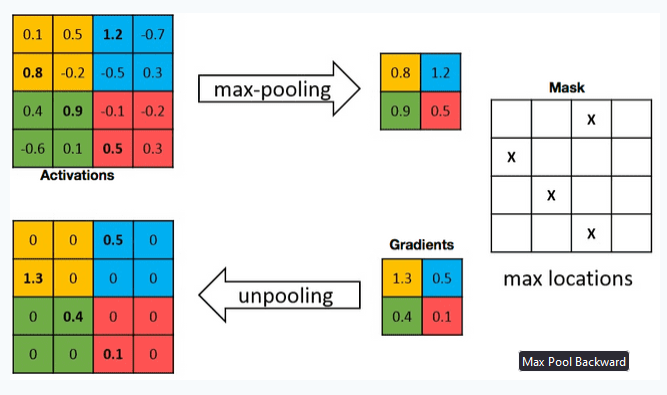
\includegraphics[width=0.9\textwidth]{pics/maxpoolback.png}
\end{frame}

\begin{frame}{Convolutional Neural Networks (CNN)}{Abschließende Bemerkungen}
   \pause
   \begin{itemize}
      \item Auch für die Upsampling-Verfahren gibt es Darstellungen die beispielsweise das Kronecker-Produkt nutzen.
   
   \pause
   \item Die Faltungsoperation muss performant implementiert werden.
   
   \pause
   \item Es sind beliebige Kombinationen möglich.

   \pause
   \item Bei der Bildklassifikation werden von CNN oft bessere Generalisierungsraten im Vergleich zu FFN erzielt.

\end{itemize}
\end{frame}

\section{Datenbankgestützte Umsetzung}
\subsection{PArADISE-Projekt}
\begin{frame}{Datenbankgestützte Umsetzung}{PArADISE-Projekt}
   \pause
   \begin{itemize}
      \item Design von Assistenzsystemen, Unterstützung der Entwickler solcher Systeme
      \pause
      \item Entwicklungsphase: Datenwisenschaftler sammeln Sensordaten, um Benutzeraktivitäten zu erkennen und vorherzusagen.
      \pause
      \item Nutzung von ML-Algorithmen, um Aktivitätsmodelle zu lernen $\rightarrow$ PaMeLA
   \end{itemize}
\end{frame}

\begin{frame}{Datenbankgestützte Umsetzung}{PaMeLA: Parallelization of Machine Learning Algorithms }
   \pause
   \begin{itemize}
      \item Anfallen großer Datenmengen, Problem: mangelnde Rechenleistung
      \pause
      \item transparente Datenbankunterstützung für Big Data Analytics
      \pause
      \item Ziel: Transformation von ML-Algorithmen in parallele SQL-Systeme
      \pause
      \item besonders interessant: Parallelisierung von Operationen der linearen Algebra
      \pause
      \item Beispiel: Hidden-Markow-Modelle, siehe Marten et. al. \cite{dissmarten}
      \pause 
      \item andere Verfahren? $\rightarrow$ FNN und CNN
   \end{itemize}
\end{frame}

\begin{frame}{Datenbankgestützte Umsetzung}{Datenbanken und SQL}
   Beispiel: 
   zwei Relationen \textbf{Angestellte} und \textbf{Projekt} als Tabellen
\begin{table}[h]
    \centering
\begin{tabular}{|c|c|c|c|c|} \hline
    \multicolumn{5}{|c|}{\textbf{Angestellte}} \\ \hline
    \hline
    ID &Name &Spezialisierung &Projektnummer &Gehalt\\ 
    \hline
    1 &Martin &Elektrotechnik &3 &2300\\ 
    \hline
    2 &Lennardt &Informatik &1 &1500\\
    \hline
    3 &Johann &Informatik &3 &1800\\
    \hline
    4 &Jana &Maschinenbau &3 &2100\\
    \hline
    5 &Antonia &Buchhaltung &2 &2000\\ 
    \hline
\end{tabular}
\caption[Beispielrelation \textbf{Angestellte}]{Abgebildet ist die Beispielrelation Angestellte mit den Attributen ID, Name, Spezialisierung, Projektnummer und Gehalt.}
\label{abb:angestellte}
\end{table}

\end{frame}

\begin{frame}{Datenbankgestützte Umsetzung}{Datenbanken und SQL}
   

\begin{table}[H]
    \centering
\begin{tabular}{|c|c|c|c|} \hline
    \multicolumn{4}{|c|}{\textbf{Projekt}} \\ \hline
    \hline
    Projektnummer &Projektname &Budget &Ort \\ 
    \hline
    1 &Datenbank 2.0 &50000 &Rostock \\ 
    \hline
    2 &Verwaltung &25000 &Rostock \\
    \hline
    3 &Forschungsabteilung  &40000 &Schwerin\\ 
    \hline
\end{tabular}
\caption[Beispielrelation \textbf{Projekt}]{Abgebildet ist die Beispielrelation Projekt mit den Attributen Projektnummer, Projektname, Budget und Ort.}
\label{abb:projekt}
\end{table}
\end{frame}

\begin{frame}{Datenbankgestützte Umsetzung}{Datenbanken und SQL}
   Eine Anfrage:
   \begin{align*}
      \label{anf:bsp}
      \begin{split}
      & \mathbf{SELECT} \; \text{A.Name, P.Projektname}\\
      & \mathbf{FROM} \; \text{Angestellte A} \; \mathbf{JOIN} \; \text{Projekt P} \\ 
      &\mathbf{ON} \; \text{A.Projektnummer} = \text{P.Projektnummer}\\
      &\mathbf{WHERE} \; \text{P.Ort}=\text{'Rostock'}
  \end{split}
  \end{align*}
\pause
  \begin{table}[H]
   \centering
\begin{tabular}{|c|c|} \hline
   \multicolumn{2}{|c|}{\textbf{Ergebnis}} \\ \hline
   \hline
   A.Name & P.Projektname \\ 
   \hline
   Lennardt &Datenbanken 2.0 \\ 
   \hline
   Antonia &Verwaltung\\
   \hline
\end{tabular}
\caption[Ergebnisrelation einer SQL-Anfrage ]{Zu sehen ist die Ergebnisrelation der zuvor beschriebenen Anfrage.}
\label{abb:result_relation}
\end{table}
\end{frame}

\begin{frame}{Datenbankgestützte Umsetzung}{Lineare Algebra und SQL}
   Ist
    \begin{equation*}
        A=\begin{pmatrix}
            1 & 2 \\
            -5 & 2 \\
            0 & 7 \\
        \end{pmatrix}
        \in \RR^{3 \times 2}
    \end{equation*}
    gegeben, \pause so ergibt sich Coordinate-Schema wie in Tabelle \ref{coordinate_scheme_table}.

\begin{table}
    \centering
    \begin{tabular}{|c|c|c|} 
        \hline
    \multicolumn{3}{|c|}{\textbf{A}} \\ \hline
     \hline
     $i$ &$j$ &$v$ \\ 
     \hline
     1 &1 &1\\ 
     \hline
     1 &2 &2\\
     \hline
     2 &1 &$-5$\\
     \hline
     2 &2 &2\\
     \hline
     3 &1 &0\\
     \hline
     3 &2 &7\\
     \hline
    \end{tabular}
    \caption[Das Coordinate-Schema]{Das Coordinate-Schema zur Matrix $A$ aus Beispiel \ref{besipiel:_coordinate_sheme}.}
    \label{coordinate_scheme_table}
\end{table}

\end{frame}

\begin{frame}{Datenbankgestützte Umsetzung}{Lineare Algebra und SQL}
   Matrixvektormultiplikation $Ax \in \RR^m$ einer Matrix $A \in \RR^{m \times n}$ und eines Vektors $x \in \RR^n$ als SQL-Anfrage

\begin{align*}
    & \mathbf{SELECT} \; A.i \; \mathbf{AS} \; i, \; \mathbf{SUM} (A.v*x.v) \; \mathbf{AS} \; v\\
    & \mathbf{FROM} \; A \; \mathbf{JOIN} \; x \; \mathbf{ON} \; A.j=x.i \; \\
    & \mathbf{GROUP} \, \mathbf{BY} \; A.i.
\end{align*}
\pause
Dabei tauchen Aggregatfunktionen und Gruppierungen auf. Andere Basisoperationen wie Skalarprodukte, Matrixmatrixmultiplikation etc. auch möglich.
\end{frame}

\begin{frame}{Datenbankgestützte Umsetzung}{Aggregate und Gruppierungen}
Sei
\begin{equation*}
    A=\begin{pmatrix}
        3 &1\\
        4 &1
    \end{pmatrix}.
\end{equation*}
Die Spaltensumme von $A$ kann mit der Gruppierungsoperation
\begin{equation*}
    \gamma_{j, \; \mathbf{SUM}(v) \rightarrow v}(\mathbf{A}) \Rightarrow 
    \begin{tabular}{|c|c|} \hline
        j &v\\
        \hline
        1 &7\\
        \hline
        2 &2\\
        \hline
    \end{tabular}
\end{equation*} 
berechnet werden.  
\begin{align*}
   & \mathbf{SELECT} \; A.j \; \mathbf{AS} \; j, \; \mathbf{SUM} (A.v) \; \mathbf{AS} \; v\\
   & \mathbf{FROM} \; A \\
   & \mathbf{GROUP} \, \mathbf{BY} \; A.j.
\end{align*}

\end{frame}

\begin{frame}{Datenbankgestützte Umsetzung}{Dünn besetzte Matrizen}
   Darstellung im Compressed-Sparse-Column-Schema ist durch 
\begin{equation*}
    A_{i,j}=\mathbf{val}[k] \Leftrightarrow (\mathbf{rowInd}[k]=i) \wedge (\mathbf{colPtr}[j] \leq k < \mathbf{colPtr}[j+1])
\end{equation*} 
gegeben. 
\pause
    Sei
    \begin{equation*}
        A=\begin{pmatrix}
            a_{11} &0 &0 &a_{14} \\
            a_{21} &a_{22} &0 &0 \\
            0 &0 &a_{33} &0 \\
            0 &a_{42} &0 &a_{44}\\
        \end{pmatrix}.
    \end{equation*}

    \begin{itemize}
        \item \textbf{val}=$[a_{11}, a_{21}, a_{22}, a_{42}, a_{33}, a_{14}, a_{44}]$,
        \item \textbf{rowInd}=$[1, 2, 2, 4, 3, 1, 4]$,
        \item \textbf{colPtr}=$[1, 3, 5, 6, 8]$.
    \end{itemize}
\end{frame}

\begin{frame}{Datenbankgestützte Umsetzung}{Dünn besetzte Matrizen}
   \begin{block}{Definition (Spaltenkompression)}
      Eine dünn besetzte Matrix $A \in \RR^{m \times n}$ wird als Relation
\begin{align*}
    \mathbf{A}(&i \; \mathrm{int} \; \mathrm{ARRAY}, \\
               &\underline{j} \; \mathrm{int}, \\
               &v \; \mathrm{double} \; \mathrm{ARRAY}
               )
\end{align*}
gespeichert. Diese Repräsentation wird Spaltenkompression genannt und ist insbesondere für die Matrixvektormultiplikation nützlich.
   \end{block}
   \pause
   Beachte: Die Array-Darstellung ist nicht in allen Systemen unterstützt.
\end{frame}
%%%%%%%%%%%% Beispielfolie zu  Auzaehlungen %%%%%%%%%%%%%%%%%%%%%%%%%%%
%%%%%%%%%%%%%%%%%%%%%%%%%%%%%%%%%%%%%%%%%%%%%%%%%%%%%%%%%%%%%%%%%%%%%%%
\subsection{Aufz\"ahlungen}
\begin{frame}{Auflistungen und Aufz\"ahlungen}
   Diese Folie hat zur Abwechslung mal keinen Untertitel, daf\"ur ist sie aber zweispaltig.

   \begin{columns}
      \column{0.45\textwidth}
         \begin{itemize}
            \item erster Auflistungspunkt
                  \begin{itemize}
                     \item n\"achste Ebene
                     \item n\"achste Ebene
                           \begin{itemize}
                              \item tiefste Ebene
                              \item tiefste Ebene
                           \end{itemize}
                     \item n\"achste Ebene
                  \end{itemize}
            \item zweiter Auflistungspunkt
         \end{itemize}

      \column{0.45\textwidth}
         \begin{enumerate}
            \item mit Aufz\"ahlungen
                  \begin{enumerate}
                     \item geht das nat\"urlich
                           \begin{enumerate}
                              \item ebenso
                              \item wie mit
                           \end{enumerate}
                     \item Auflistungen
                  \end{enumerate}
         \end{enumerate}
   \end{columns}

\end{frame}


%%%%%%%%%%%% Beispielfolie zu Boxen etc.    %%%%%%%%%%%%%%%%%%%%%%%%%%%
%%%%%%%%%%%%%%%%%%%%%%%%%%%%%%%%%%%%%%%%%%%%%%%%%%%%%%%%%%%%%%%%%%%%%%%
\subsection{Theorem / Beweis / andere Boxen} 

\begin{frame}[allowframebreaks]{Theorem / Beweis / andere Boxen} % Dieses Frame wird je nach Platz/Inhalt/Fuellstand automatisch geteilt
   \begin{theorem}
      Diese Box ist sch\"on.
   \end{theorem}

   \begin{proof}
      Die CD-Vorlage ist insgesamt schick, ergo muss jedes Teil hiervon dekorativ sein, folglich also auch die obige Theorem-Box.
   \end{proof}

   \begin{Beispiel}
     Diese Box ist auch ein nettes Beispiel f\"ur schicke Boxen.
   \end{Beispiel}

   \begin{block}{Blocktitel}
      Ein Block mit dem Titel \insertblocktitle
   \end{block}

   \begin{alertblock}{Alertblocktitel}
      Ein Alertblock.
   \end{alertblock}

   \begin{exampleblock}{Beispielblocktitel}
      Ein Beispielblock.
   \end{exampleblock}

\end{frame}

%%%%%%%%%%%% Details zum Style %%%%%%%%%%%%%%%%%%%%%%%%%%%%%%%%%%%%%%%%
%%%%%%%%%%%%%%%%%%%%%%%%%%%%%%%%%%%%%%%%%%%%%%%%%%%%%%%%%%%%%%%%%%%%%%%
\section{Details zum Uni Rostock Style}

%%%%%%%%%%%% Inhaltsverzeichnis mal zeigen %%%%%%%%%%%%%%%%%%%%%%%%%%%%
%%%%%%%%%%%%%%%%%%%%%%%%%%%%%%%%%%%%%%%%%%%%%%%%%%%%%%%%%%%%%%%%%%%%%%%
\frame{\tableofcontents[currentsection]}

\subsection{Einbindung des Styles}
\begin{frame}[fragile]{Einbindung des Styles}% [fragile] weil es sonst Probleme mit der verbatim-Umgebung gibt
   Alle f\"ur das Style notwendigen Dateien liegen im Unterordner \texttt{./unirostock}.
   Das Stylefile selbst kann mittels
   \begin{verbatim}
\usepackage[mnf,footuni]{./unirostock/beamerthemeRostock}
   \end{verbatim}\vspace*{-0.5cm}
   eingebunden werden. Der erste Parameter ist das Fakult\"atsk\"urzel, das das Farbschema vorgibt.
   M\"ogliche Werte sind \texttt{uni, inf, msf, ief, mnf, mef, juf, wsf, auf, thf, phf}.

   Der zweite Parameter steuert das Verhalten der Fu{\ss}zeile:
   \begin{tabular}{lp{0.8\textwidth}}
     \texttt{footuni}   & Fu{\ss}zeile wie im CD-Handbuch (Standard)\\
     \texttt{foottitle} & Autor und Kurztitel in der Fu{\ss}zeile \\
     \texttt{footheadings} & Abschnitt und Unterabschnitt in der Fu{\ss}zeile \\
     \texttt{footuniheadings} & Author und Uni sowie Abschnitt und Unterabschnitt
   \end{tabular}
\end{frame}


%%%%%%%%%%%% Details zum Style %%%%%%%%%%%%%%%%%%%%%%%%%%%%%%%%%%%%%%%%
%%%%%%%%%%%%%%%%%%%%%%%%%%%%%%%%%%%%%%%%%%%%%%%%%%%%%%%%%%%%%%%%%%%%%%%
\subsection{\LaTeX und pdf\LaTeX}
\begin{frame}[fragile]{\LaTeX und pdf\LaTeX}
  Da zur Erstellung der Foliendekoration das (sowieso mit der \verb+beamer+-class eingebundene) Paket \verb+pgfgraphics+ zur Anwendung kam, k\"onnen die mit diesem Style erstellten Vortr\"age sowohl mittels
  \begin{verbatim}
pdflatex beamer_sample.tex
  \end{verbatim}
  als auch mit
  \begin{verbatim}
latex beamer_sample.tex
dvips beamer_sample.dvi
ps2pdf beamer_sample.ps
  \end{verbatim}
  \"ubersetzt werden. Es gelten nat\"urlich die \"ublichen Regeln bez\"uglich der erlaubten Grafikformate bei Verwendung von pdf\LaTeX bzw.\LaTeX.
\end{frame}


%%%%%%%%%%%% Farbschema %%%%%%%%%%%%%%%%%%%%%%%%%%%%%%%%%%%%%%%%%%%%%%%
%%%%%%%%%%%%%%%%%%%%%%%%%%%%%%%%%%%%%%%%%%%%%%%%%%%%%%%%%%%%%%%%%%%%%%%
\subsection{Farbschema}
\begin{frame}[fragile]{Farbschema}{Tolle Automatik}
   Das Farbschema wird komplett durch den Fakult\"atsparameter bei der Einbindung des Styles bestimmt. Es empfiehlt sich, bei Grafiken, Tabellen ein entsprechend passendes Schema zu w\"ahlen.

   Das Hintergrundbild auf der Titelseite wird auch automatisch eingebunden. Es ist jedoch nicht vorgeschrieben und kann (und sollte) nach eigenem Bedarf ersetzt werden. Hierzu dient der Befehle \verb+\titleimage{..}+. Weitere Details hierzu finden sich im Quellcode des Beispieldokumentes und auf der \"ubern\"achsten Folie. Bei manueller Wahl eines Hintergrundbildes empfiehlt sich, auf einen guten Pass zum Farbschema zu achten.
\end{frame}


%%%%%%%%%%%% Farbschema %%%%%%%%%%%%%%%%%%%%%%%%%%%%%%%%%%%%%%%%%%%%%%%
%%%%%%%%%%%%%%%%%%%%%%%%%%%%%%%%%%%%%%%%%%%%%%%%%%%%%%%%%%%%%%%%%%%%%%%
\subsection{Tabellen}
\begin{frame}[fragile]{Tabellenfarben}
   Dei Befehle \verb+\zfA+, \verb+\zfB+, \verb+\zfC+, \verb+\zfD+ stellen einen effektiven Weg dar, um die Zeilenfarbe in Tabellen anzupassen. Sie werden einfach vor die Tabellenzeile gestzt, also zum Beispiel
   \begin{verbatim}
\zfA Spalte1 & spalte2 & ..
   \end{verbatim}
   Intern wird mit dem Befehl \verb+\rowcolor{..}+ des Paketes \texttt{colortbl} gearbeitet. Es empfiehlt sich ein Blick in dessen Dokumentation f\"ur fortgeschrittene Anwendungen.

   \begin{center}
   \begin{tabular}{ccc}
      \zfA Zeilenfarbe A & gew\"ahlt mit dem Befehl & \verb+\zfA+ \\
      \zfB Zeilenfarbe B & gew\"ahlt mit dem Befehl & \verb+\zfB+ \\
      \zfC Zeilenfarbe C & gew\"ahlt mit dem Befehl & \verb+\zfC+ \\
      \zfD Zeilenfarbe D & gew\"ahlt mit dem Befehl & \verb+\zfD+
   \end{tabular}
   \end{center}
\end{frame}


%%%%%%%%%%%% Titelseite %%%%%%%%%%%%%%%%%%%%%%%%%%%%%%%%%%%%%%%%%%%%%%%
%%%%%%%%%%%%%%%%%%%%%%%%%%%%%%%%%%%%%%%%%%%%%%%%%%%%%%%%%%%%%%%%%%%%%%%
\subsection{Einstellungen f\"ur die Titelseite}
\begin{frame}[fragile]{Befehle f\"ur die Titelseite I}
  \begin{itemize}
  \item Vortragstitel:
  \begin{verbatim}
\title[Kurztitel (f\"ur die Fu{\ss}zeile)]{Langer Titel}
  \end{verbatim}

  \item Untertitel:
  \begin{verbatim}
\subtitle{Untertitel}
  \end{verbatim}

  \item Autor(en):
  \begin{verbatim}
\author{Name}
  \end{verbatim}

  \item Einrichtung / Institut / Universit\"at:
  \begin{verbatim}
\institute{Universit\"at Rostock, Institut f\"ur Physik}
  \end{verbatim}
  \end{itemize}
\end{frame}

\begin{frame}[fragile]{Befehle f\"ur die Titelseite II}
  \begin{itemize}
  \item Zus\"atzlich gibt es Platz f\"ur eigene Eintr\"age, ein Logo oder \"ahnliches mittels
  \begin{verbatim}
\titlegraphic{Zusatztext}
  \end{verbatim}
   Dabei kann beliebiger \LaTeX-Code \"ubergeben werden, also auch \verb+\includegraphics{..}+, \verb+\centering+ etc.
  \item Ein eigenes Titelbild kann mit
  \begin{verbatim}
\titleimage{dateiname.xyz}
  \end{verbatim}
  eingebunden werden. Die Skalierung und das Abschneiden der oberen rechten Ecke erfolgen automatisch. Wichtig ist, ein sinnvolles Seitenverh\"altnis der Originalgraphik zu w\"ahlen, um Verzerrung zu vermeiden und au{\ss}erdem das Bild \"uber Kontrast und Helligkeit entsprechend blass einzustellen.
  \end{itemize}
\end{frame}


%%%%%%%%%%%% kopf- und Fusszeile %%%%%%%%%%%%%%%%%%%%%%%%%%%%%%%%%%%%%%
%%%%%%%%%%%%%%%%%%%%%%%%%%%%%%%%%%%%%%%%%%%%%%%%%%%%%%%%%%%%%%%%%%%%%%%
\subsection{Einstellungen f\"ur Kopf- und Fu{\ss}zeile}
\begin{frame}[fragile]{Kopf- und Fu{\ss}zeile}
   \begin{itemize}
      \item Der Institutsname f\"ur die Fu{\ss}zeile wird mit
      \begin{verbatim}
 \footinstitute{Fakult\"at, Institut}
      \end{verbatim}
            angepasst. Er wird nur angezeigt, wenn bei Paketeinbindung der Parameter \verb+footuni+ angegeben ist.

      \item Der Logobereich oben rechts kann mittels
      \begin{verbatim}
\renewcommand{\mylogo}{\includegraphics[
                     width=18.5mm]{institutslogo}}
      \end{verbatim}
      angepasst werden. Dies ist der in diesem Dokument benutzte Beispielcode. Erlaubt sind alle Minipage-vertr\"aglichen \LaTeX-Befehle.
   \end{itemize}
\end{frame}


%%%%%%%%%%%% Allgemeines %%%%%%%%%%%%%%%%%%%%%%%%%%%%%%%%%%%%%%%%%%%%%%
%%%%%%%%%%%%%%%%%%%%%%%%%%%%%%%%%%%%%%%%%%%%%%%%%%%%%%%%%%%%%%%%%%%%%%%
\section{Allgemeines}
\frame{\tableofcontents[currentsection]}

\begin{frame}{Allgemeine Bemerkungen}
   \paragraph{Hinweise zum Design}
   Diese Beispielpr\"asentation ist reichlich \"uberladen, um alle Features zu demonstrieren. Es ist empfehlenswert, die eigene Pr\"asentation kritisch zu hinterfragen in Bezug auf die F\"ulle der Folien, ihre Anzahl und Gestaltung sowie die Einhaltung der allgemeinen Regeln f\"ur Pr\"asentationen.

   \paragraph{Wirklich letzter Hinweis}
   Viele Fragen lassen sich beim Blick in den Quellcode dieser Beispielpr\"asentation kl\"aren. Insbesondere die (zugegebenerma{ss}en sparsam verteilten) Kommentare k\"onnten hilfreich sein. Ebenso ist ein Blick in \href{http://www.ctan.org/tex-archive/macros/latex/contrib/beamer/doc/beameruserguide.pdf}{\texttt{\underline{beamerusersguide.pdf}}} immer zu empfehlen. Und ein zweiter Blick auch ;-)
\end{frame}


%%%%%%%%%%%% Schluss jetzt %%%%%%%%%%%%%%%%%%%%%%%%%%%%%%%%%%%%%%%%%%%%
%%%%%%%%%%%%%%%%%%%%%%%%%%%%%%%%%%%%%%%%%%%%%%%%%%%%%%%%%%%%%%%%%%%%%%%
\end{document}

